\subsection{Théorie}

\subsubsection{Qu'est-ce que la pupinisation? Pourquoi n'est-ce plus utilisé?}

La pupinisation consiste à augmenter artificiellement l'impédance de la
ligne en insérant en série des inductances à intervalles réguliers et en créant
un filtre passe-bas pour uniformiser l'inductance électrique de la
ligne. \newline

Cette technique permet de compenser la forte capacité du câble et ainsi
d'améliorer la portée du signal. Ce n'est plus utilisé de nos jours car
cela ne fonctionne que pour les basses fréquences (forte atténuation sur
les hautes fréquences), jusqu'à environ 3.4KHz ce qui limite fortement
la bande passante. Or, ces hautes fréquences sont utilisées par des
technologies comme l'ADSL. \newline

On exprime l'impédance caractéristique d'une ligne comme étant 
$$Z_c = \sqrt{\frac{R + j\omega L}{G + j\omega C}}$$
Et l'on exprime l'exposant de propagation $\gamma$ avec $\alpha$ l'atténuation et $\beta$ le déphasage comme étant
$$\gamma = \sqrt{(R + j\omega L)(G + j\omega C)} = \alpha + j\beta$$

Dans une ligne on suppose G comme étant nul, si dans notre ligne nous
avons la résistance $R$ qui est nettement plus grande que l'inductance
$L$ (cas 1), alors nous avons:
$$\gamma = \sqrt{\frac{\omega RC}{2}} + j\sqrt{\frac{\omega RC}{2}}$$
$$Z_c = \sqrt{\frac{R}{j\omega C}}$$
Nous obtenons donc que l'atténuation et le déphasage sont directement
proportionnels à la fréquence du signal et l'impédance caractéristique
de la ligne qui est inversément proportionnelles à celle-ci (car $\omega
= 2\pi f$). \newline

Si par contre dans notre ligne nous avons la résistance $R$ qui est
nettement plus petite que l'inductance $L$ (cas 2), nous obtenons le résultat suivant:
$$\gamma = \frac{R}{2}\sqrt{\frac{C}{L}} + j\omega \sqrt{LC}$$
$$Z_c = \sqrt{\frac{L}{C}}$$
Ce qui nous donne une impédance et une attenuation indépendante du
signal et un déphasage qui dépend de la fréquence. \newline 

En augmentant artificiellement l'impédance de la ligne (pupinisation)
on évite de se retrouver dans le premier cas. Le second cas correspond à
$\omega L >> R$ qui correspond à celui d'un fil avec peu de résistance et
qui représente une bonne situation pour une ligne.\newline

\subsubsection{Comment caractérise-t-on la directivité d'une antenne? Donnez un
exemple d'application où l'on veut une antenne directive et non directive.}

La directivité d'une antenne est caractérisée par la façon dont elle
rayonne. Si elle rayonne de la même façon dans toutes les directions du
plan horizontal, on dit qu'elle est équidirective et on parle alors
d'antenne isotrope. \newline

Si par contre, elle possède un ou 2 lobes nettement plus importants que
les autres (les lobes principaux), on dit qu'elle est directive. Elle
l'est d'autant plus que le lobe le plus important est étroit
(c'est-à-dire que son angle d'ouverture est petit). \newline

\begin{description}
    \item[Antennes directives] : antennes paraboliques (type Yagi)
    \item[Antennes non directives] : antenne GSM, antenne WiFi
\end{description}

\bigskip

Dans la vie de tous les jours, on préférera avoir une antenne non
directive (avec un angle d'ouverture le plus large possible) lorsque les
stations avec lesquelles on doit communiquer peuvent se déplacer comme
les GSM, les récepteurs WiFi. A contrario, on préfèrera avoir une
antenne directive (avec un angle d'ouverture le plus faible possible)
lorsqu'on sait que l'émetteur et le récepteur ne bougeront pas du jour
au lendemain, on se focalise dans la bonne direction, ce qui permet de
réduire le bruit du signal (comme les antennes paraboliques pour la télévision).

\subsubsection{Décrivez un type de modulation analogique au choix}

\paragraph{La modulation de fréquence}

Cette modulation (FM) consiste à modifier la fréquence du signal à
transmettre en l'augmentant ou la diminuant en fonction de la porteuse.
Si la porteuse (c'est-à-dire la fréquence du signal porteur) est
positive, la fréquence sera augmentée et les sinusoïdes seront plus
rapprochées. \newline

La modulation de fréquence est plus robuste que la modulation
d'amplitude pour transmettre un mesage dans des conditions difficiles
(atténuation et bruit importants).

Exemples d'utilisation :
\begin{itemize}
    \item Les modems bas débit
    \item Les téléphones analogiques
    \item Les radios de la bande FM
    \item Certains synthétiseurs
\end{itemize}

\begin{center}
    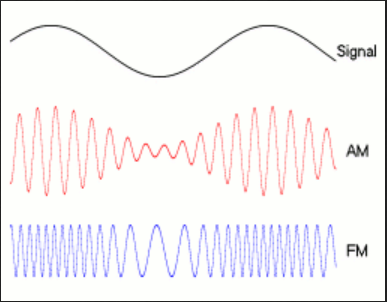
\includegraphics[width=0.5\linewidth]{img/modulation_am_fm.png}
\end{center}

\paragraph{La modulation d'amplitude}

Soit la porteuse $v(t) = A_c cos(\omega_c t + \varphi_c)$, pour avoir une modulation d'amplitude nous allons ajouter le signal \textit{modulant} $m(t)$ multiplié par un \textit{indice de modulation} $k$ à ce signal.
$$s(t) = [1+km(t)] A_c cos(\omega_c t + \varphi_c)$$
Il s'agit donc d'une modulation d'amplitude (AM), ou l'amplitude va
varier en fonction du signal modulant. Il faut bien faire attention dans
le choix de l'indice de modulation (entre 0 et 100\%), pour éviter la surmodulation. En
effet un indice trop élevé pourrait causer un renversement de phase
ce qui pourrait causer de l'ambiguïté lors de la démodulation. \newline

Pour démoduler ce type de modulation on va multiplier le signal modulé par la porteuse (elle doit être disponible à l'émission et à la réception), nous aurons ainsi
\begin{eqnarray*}
A_c s(t)cos(\omega_c t + \varphi_c)*cos(\omega_c t + \varphi_c) &=&A_c s(t)cos^2(\omega_c t + \varphi_c)\\
&=& A_c s(t) \frac{1+ cos(2\omega_c t + 2\varphi_c)}{2}\\
&=& \frac{A_cs(t)}{2} + \frac{A_cs(t)cos(2\omega_c t + 2\varphi_c)}{2}
\end{eqnarray*}
Un filtrage passe bas nous laissera le signal démodulé. \newline

La modulation va aussi créer deux bandes de même taille à gauche et à droite de la porteuse, on voit ca en convertissant le signal du temporel au fréquentiel
$$f(t) cos(\omega_0 t) \Leftrightarrow \frac{F(\omega - \omega_0) + F(\omega + \omega_0)}{2}$$
Dès lors il va falloir choisir combien de bande conserver (en effet il y
a doublon dans l'information). Dès lors plusieurs modes existent :
\begin{itemize}
\item DSB (doubleside band): envoi des deux bandes
\item LSB (lowerside band): on envoi les deux bandes intérieures
\item USB (upperside band): on envoi les deux bandes extérieure
\item QAM (bande latérale unique): on transforme le signal $m(t)$ en
    deux signaux $s_1(t)$ et $s_2(t)$ et l'on envoi $s(t) = s_1(t)
    cos(\omega_c t) + s_2(t) sin(\omega_c t)$. Ainsi une démodulation
    avec $cos(\omega_c t)$ nous fournira $s_1(t)$ et une démodulation
    avec $sin(\omega_c t)$ nous fournira $s_2(t)$. 
\item VSB (vestigialside band): il s'agit d'un envoi en bande latérale
    résiduelle, quand une fréquence est trop près de 0 Hz on ne peut pas
    envoyer une bande latérale unique, on va alors atténuer au maximum
    l'un des cotés.
\end{itemize}

La modulation d'amplitude a un niveau de bruit constant assez élevé. 

\begin{figure}[H]
    \centering
    \begin{minipage}[t]{0.45\linewidth}
        \centering
        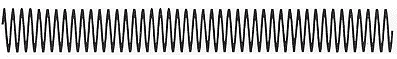
\includegraphics[width=0.75\linewidth]{img/signal_porteur.png}
        \caption{Porteuse (signal porteur)}
    \end{minipage}
    \begin{minipage}[t]{0.45\linewidth}
        \centering
        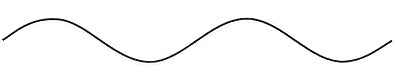
\includegraphics[width=0.75\linewidth]{img/signal_modulant.png}
        \caption{Signal modulant}
    \end{minipage}
\end{figure}

\begin{figure}[H]
    \begin{center}
        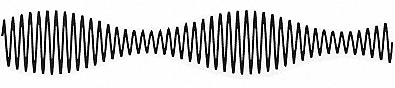
\includegraphics[width=0.335\linewidth]{img/signal_module.png}
        \caption{Signal modulé}
    \end{center}
\end{figure}

\begin{figure}[H]
    \begin{center}
        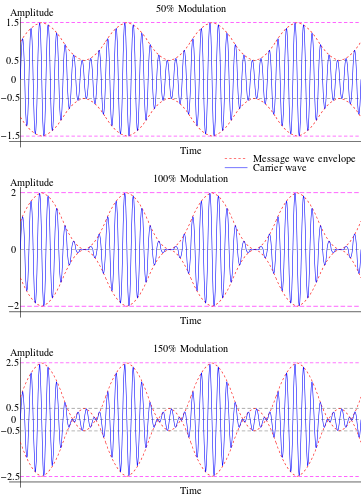
\includegraphics[width=0.5\linewidth]{img/indice_de_modulation_AM.png}
        \caption{Signal modulé selon différents indices de modulation}
    \end{center}
\end{figure}

Comme le démodulateur lit la partie haute du signal, le signal (à cause
de l'indice de modulation trop haut) devient négatif mais le
démodulateur lira un signal positif et disposera alors d'informations
eronnées. \newline

\subsubsection{Décrivez le rôle des différents blocs du schéma de modulation digitale ci dessous.}
\begin{figure}[H]
  \centering
  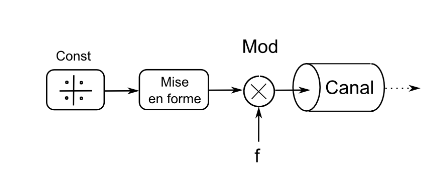
\includegraphics[width=10cm]{img/exo.png}
  \caption{Elements de la modulation digitale}
\end{figure}

\paragraph{Const} ou \textit{mapping du signal}. On transforme
la séquence de bits en séquence de symboles complexes. Il y a 2 axes,
celui des réels (I) et celui des imaginaires (Q). On choisit  ensuite la
constellation suivant le débit voulu, tout en faisant attention au bruit
car la probabilité d'erreurs sur une QAM-16 est plus élevée que sur une
QAM-4. Enfin, si on utilise le mapping de Gray, on veille à ce qu'il n'y
ait qu'un seul bit de différence entre les points les + proches.
\newline

\begin{figure}[H]
    \centering
    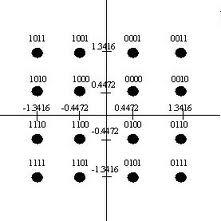
\includegraphics[width=0.5\linewidth]{img/mapping.png}
    \caption{Exemple de mapping}
\end{figure}

\paragraph{Mise en forme} Grâce au passage par Const, on sait que le
nombre d'inputs possibles est fini, assurant qu'on peut assigner à
chaque input une certaine valeur sous forme de courant pour créer le
signal. Chaque input sera transmis pendant un intervalle de temps T qui
correspond à la fréquence d'échantillonage.
Cette mise en forme est rectangulaire (une certaine tension pendant
une certaine durée) et \og{}abrupte\fg{} puisqu'elle provoque
des passages de courant de +1V à -1V instantanément (irréalisable en
pratique). En pratique, le passage entre les différentes tensions se
fait sur une durée plus longue, ceci peut provoquer l'ISI (Inter Symbol
Interference) qui consiste à l'incompréhension du signal par le
récepteur. Pour éviter cette situation, on applique le critère de
Nyquist qui consiste à échantilloner au milieu du moment (chaque T/2) où le signal a
été envoyé, qui correspond normalement à l'endroit qui a le plus de
chance de contenir la valeur que l'émetteur souhaitait transmettre. Pour
que ce critère fonctionne, il faut une bonne synchronisation entre
l'émetteur et le récepteur, que la mise en forme respecte le principe de
superposition (c'est-à-dire soit linéaire : la somme de deux entrées
quelconques égale à la somme de deux sorties quelconques ; le multiple
d'une entrée quelconque correspond au multiple de la sortie
correspondante) ainsi que peu de dispersion sur le signal.\newline

On peut décider de garder une seule partie du signal grâce à un filtre
passe-bas (garder les basses fréquences), un filtre passe-haut (garder
les hautes fréquences) ou un filtre passe bande (garder une certaine
bande de fréquence). \newline

\paragraph{Modulateur de fréquence}

La modulation (FM) consiste à modifier la fréquence du signal à
transmettre en l'augmentant ou la diminuant en fonction de la porteuse.
Si la porteuse (c'est-à-dire la fréquence du signal porteur) est
positive, la fréquence sera augmentée et les sinusoïdes seront plus
rapprochées. \newline

La modulation de fréquence est plus robuste que la modulation
d'amplitude pour transmettre un mesage dans des conditions difficiles
(atténuation et bruit importants).

Exemples d'utilisation :
\begin{itemize}
    \item Les modems bas débit
    \item Les téléphones analogiques
    \item Les radios de la bande FM
    \item Certains synthétiseurs
\end{itemize}

\begin{center}
    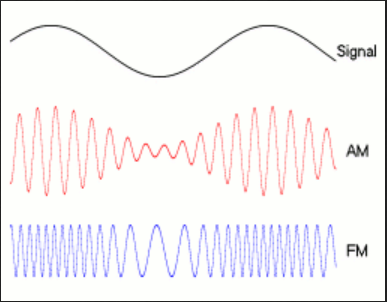
\includegraphics[width=0.5\linewidth]{img/modulation_am_fm.png}
\end{center}


\subsubsection{Quel est le principe du CDMA ? Deux exemples d'options alternatives pour
implémenter la division de l'accès pour les différents utilisateurs.}

Le CDMA (code division multiple access) attribue un code (une sorte
d'identifiant) à chaque personne qui communique sur le canal pour lui
permettre de communiquer simultanément sur la même fréquence porteuse.
Chaque code est différent et il y a une très faible corrélation entre
les différents codes, ce qui permet à l'émetteur de créer un seul signal
qui contient les informations pour tous les utilisateurs et aux
utilisateurs de décoder ce signal en faisant une multiplication avec
leur code. Ce mécanisme fonctionne très bien quand il y a peu
d'utilisateurs sur le réseau et il permet à chacun de profiter de la
totalité de la bande passante.\newline

Une première alternative est le TDMA qui divise la bande passante en
un ensemble de timeslot que les différents utilisateurs vont pouvoir
utiliser, ce qui limite l'usage de chaque utilisateur à un certain
temps. Cette technique est un multiplexage temporel où la même fréquence
est attribuée à différents utilisateurs qui se partagent le temps selon
les time slices.\newline

Une seconde alternative est le FDMA qui permet de séparer le canal en un ensemble de canaux de
fréquence indépendants. Il faut faire attention dans ce type de
multiplexage que les canaux soit bien séparé. Chaque utilisateur a donc
une bande de fréquence différente.\newline

\begin{figure}[H]
    \centering
    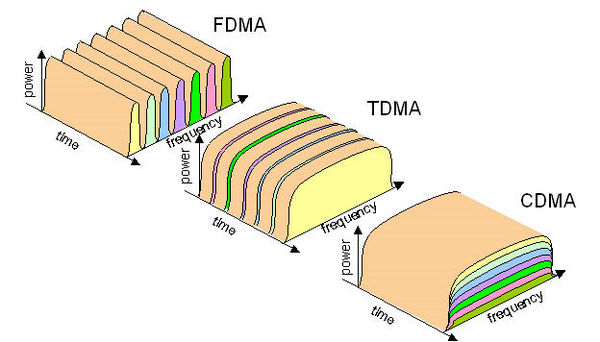
\includegraphics[width=0.65\linewidth]{img/fdma_tdma_cdma.png}
    \caption{Différence entre le FDMA, TDMA et CDMA}
\end{figure}

\subsubsection{Qu'est-ce que le mécanisme ARQ? Pourquoi est il parfois
    utilisé à la place des correcteurs d'erreurs et quand ?}

Le mécanisme ARQ est un mécanisme de contrôle d'erreurs utilisé quand on
désire une plus grande fiabilité dans les communications. Il se base sur
des acquittements (ACK) envoyés du récepteur à l'émetteur.
Il s'agit d'un système de transmission de
données appartenant à la couche Liaison (niveau 2) du modèle OSI. Il
existe plusieurs modes à ce système de transmission.
\begin{itemize}
\item \textbf{Stop-and-wait} A chaque paquet de données envoyé
    l'émetteur attend une confirmation (ACK) du récepteur. Si il y a une
    erreur, l'émetteur renvoie le paquet. 
\item \textbf{Go-back-n} L'émetteur envoie un certain nombre de ses paquets sans attendre la
    réponse de l'utilisateur. S'il reçoit sur un acquittement contenant un
    nombre ne correspondant pas à celui de la dernière trame envoyée, ce
    nombre identifie le premier paquet manquant et l'émetteur redémarre l'envoi à partir de
    celui-ci. Dès que le récepteur voit une
    erreur il arrête de récupérer des paquets.
\item \textbf{Selective-repeat} Lorsqu'une erreur intervient le
    récepteur prévient l'émetteur en lui disant quel paquet a foiré,
    mais il continue à récuperer les paquets. A un moment l'emetteur va
    renvoyer le paquet manquant en question.
\end{itemize}

\begin{figure}[H]
    \centering
    \begin{minipage}[t]{0.3\linewidth}
        \centering
        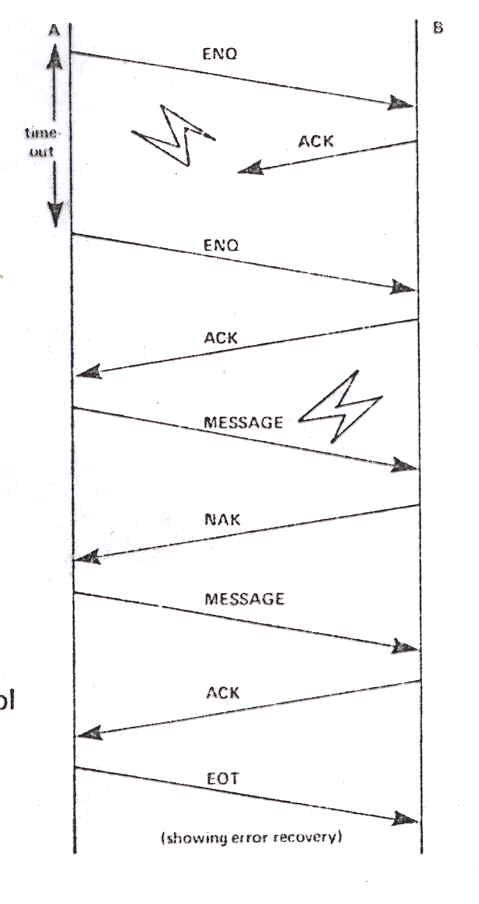
\includegraphics[width=\linewidth]{img/stop_and_wait.png}
        \caption{Stop and wait}
    \end{minipage}
    \begin{minipage}[b]{0.6\linewidth}
        \centering
        \begin{minipage}[t]{\linewidth}
            \centering
            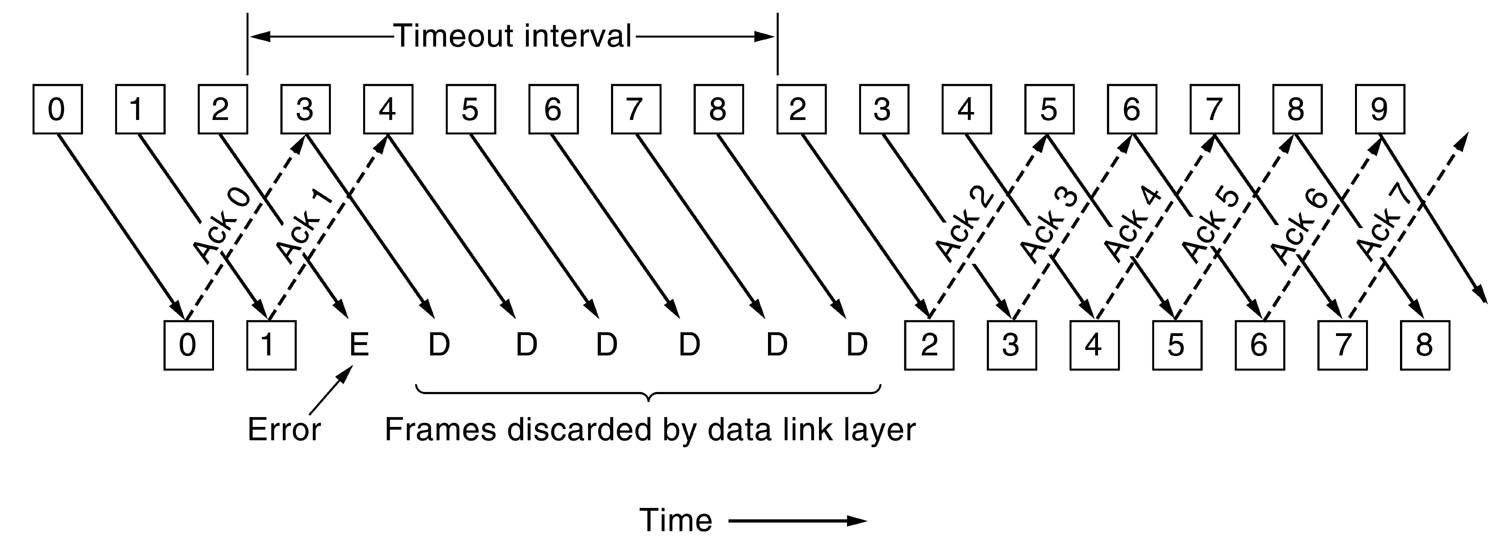
\includegraphics[width=\linewidth]{img/go_back_n.png}
            \caption{Go-back-n}
        \end{minipage}
        \begin{minipage}[b]{\linewidth}
            \centering
            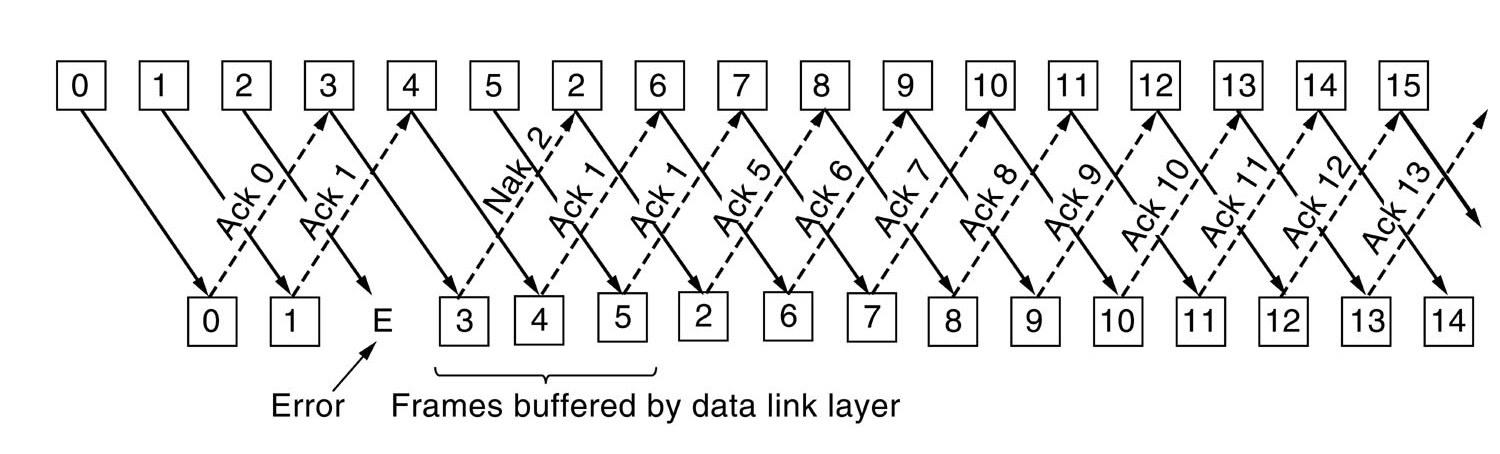
\includegraphics[width=\linewidth]{img/selective_repeat.png}
            \caption{Selective repeat}
        \end{minipage}
    \end{minipage}
\end{figure}

Le mécanisme ARQ est utilisé parfois à
la place des codes correcteurs d'erreurs tout simplement parce que dans
certains cas utiliser un code correcteur d'erreurs est simplement trop
couteux. En effet, supposons que l'on veut envoyer $10^6$ bits par
blocs de 1000bits. Si on a une ligne T1 de transmission avec un taux d'erreur (BER) de
$10^{-6}$ (sur 1 millions de bit, il y en un seul fautif)
et une ligne T2 avec un taux d'erreur de $10^{-4}$. \\
Si on utilise un code(1010,1000) pour corriger les erreurs simples. On a
besoin de 10000 bits de contrôle (car on a 1000 blocs)
cela pour T1 et T2.

Par contre si utilise un code(1001,1000) pour détecter les erreurs (par exemple la parité):
\begin{itemize}
\item Dans T1,  pour les 1000 blocs, on aura envoyé les 1000 bits de
    contrôle + la répétition des 1001 bits du blocs qui contient le bit
    eronné, on a donc ajouté 2001 bits (raisonnable).
\item Dans T2, on aura aussi envoyé 1000 bits de contrôle mais en plus
    la répétiion des 100*10001 bits des blocs erronés (le 100 vient du fait que sur les $10^6$ bits il y en a 100 fautifs). On aura donc ajouter en tout avec notre code détecteurs d'erreurs plus de 100 000 bits.
\end{itemize}

En conclusion, si le taux d'erreur est faible, il est plus intéressant
de renvoyer un paquet de temps en temps plutôt que d'ajouter énormément
de répétition pour s'assurer de la reconstruction des paquets en cas
d'erreur. \newline

\subsubsection{Quel est l'interêt de la DCT dans le codage JPEG? La DCT est elle une
opération avec ou sans pertes ?}

La DCT est une transformée de Fourier avec cosinus qui permet de
remplacer une matrice $8\times 8$ pixels contenant de la luminance en
une matrice de $8\times 8$ coefficients DCT contenant exactement la même
information. Cette application de Fourier est sans pertes, cependant son
intérêt réside dans le fait que certains coefficients sont moins
importants que d'autres. \newline

Il s'agit des coefficients à hautes fréquences
(situés en haut à gauche de la matrice) qui sont réservés à des
changements rapides d'intensité du pixel (contraste élevé), généralement invisible à
l'\oe il nu. On peut omettre certains de ces coefficients sans risquer
une grosse perte de qualité pour l'\oe il humain, ce qui
permet de faire une compression, celle-ci se fait donc avec pertes
puisqu'on ne pourra jamais retrouver les coefficients négligés.

\subsubsection{Qu'est-ce que l'alignement temporel dans le système GSM? Pourquoi
est-il seulement nécessaire dans la liaison montante?}

Le système GSM utilise la technologie TDMA, cette technologie consiste à
allouer à chaque utilisateur un time slot particulier lors duquel il
peut utiliser la fréquence. Lorsqu'un utilisateur passe un appel avec
son GSM, il peut se déplacer et donc changer sa distance par rapport à
l'antenne, changeant ainsi le temps qu'il met à la joindre par onde. Ce
changement de distance (et de délai) peut provoquer un overlap des time
slots alloués aux utilisateurs créant ainsi des interférences.\newline

Pour éviter cette situation, on a introduit l'alignement temporel qui
consiste à adapter la réception en faisant un décalage de bits pour
rester dans le bon timeslot. C'est uniquement nécessaire dans la liaison
montante car c'est le GSM qui fait le décalage, pas l'antenne. \newline

\subsubsection{Qu'est-ce qu'un algorithme de cryptographique à clé publique?
Dans quel cadre est-il généralement utilisé? Quels sont ses désavantages?}

Un algorithme à clé publique (ou asymétrique) correspond à un algorithme
de cryptographie utilisant 2 types de clés. \newline

Supposons A et B, deux personnes souhaitant s'envoyer des messages dont
ils souhaitent garder le contenu secret. Les messages vont être cryptées
mathématiquement par des fonctions à sens unique, telles qu'elles
nécessitent les informations de deux clés pour retrouver la formule à
partir de la solution. Parmi ces deux clés, A va en garder une secrète
(c'est une clé privée) et va en envoyer une à B. B va crypter ses
messages à l'aide de la clé publique, les rendant lisible uniquement par
quelqu'un qui aurait la \og{}clé publique\fg{}, sorte de brèche secrète
de l'équation. De cette manière, quelqu'un qui intercepterait la clé
publique et/ou les messages entre A et B serait incapable de les
comprendre sans avoir accès à la clé privée.\newline

Ce chiffrement est plus lent, plus difficile et les clés doivent être plus
longues pour assurer un même niveau de sécurité qu'avec la cryptographie
symétrique. La véritable difficulté est d'être sûr que le créateur de la
clé publique n'est pas un utilisateur autre que A (malveillant) qui
l'aurait communiqué à B, ce qui demande des certifications de clés
publiques. \newline

\begin{figure}[H]
    \centering
    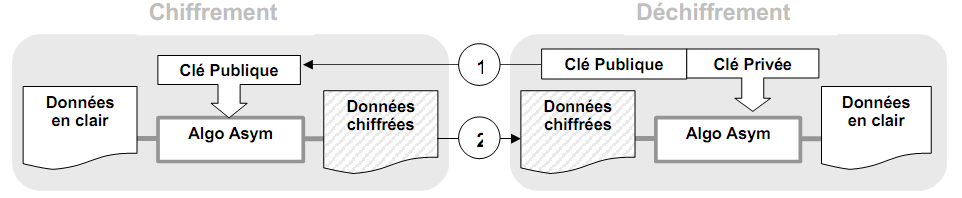
\includegraphics[width=\linewidth]{img/algorithme_asymetrique.png}
    \caption{Schéma d'utilisation d'un algorithme asymétrique}
\end{figure}

\subsubsection{Qu'est-ce la distorsion et à quoi est-ce dû ?}

La distorsion (ou \textit{dispersion}) correspond à une des
caractéristiques des lignes, c'est l'ensemble des modifications
indésirables d'un signal (sauf gain/atténuation/retard). \newline

Concrètement, il s'agit d'une déformation non-linéaire d'un signal (majoritairement
les signaux analogiques) qui peut être par exemple provoqué par la
présence d'une harmonique (le plus souvent une harmonique de rang 3) qui
s'ajoute au signal. Comme un signal peut toujours se décomposer en une
somme de sinusoïde, la troisième harmonique et le signal de base vont
constituer un nouveau signal qui ne permettra pas de retrouver le signal
original. \newline

\begin{figure}[H]
    \centering
    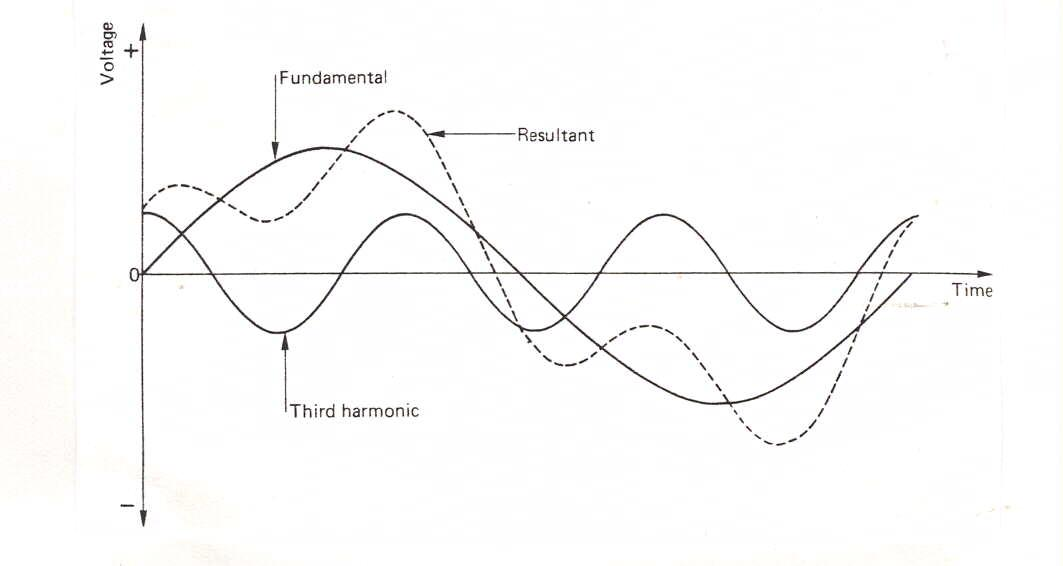
\includegraphics[width=0.7\linewidth]{img/dispersion.png}
    \caption{Exemple de dispersion}
\end{figure}

\subsubsection{Qu'est-ce que l'atténuation et à quoi est-ce dû ?}

L'atténuation est la diminution de l'amplitude ou de la puissance d'un
signal lors de sa transmission. Elle est dûe à la distance (la puissance
d'un signal diminue de manière exponentielle) et est donc un facteur
limitatif dans les télécommunications. \newline

Idée :
\[
    \textrm{Atténuation} = \frac{\textrm{valeur en
    sortie}}{\textrm{valeur en entrée}}
\]
\bigskip

Calcul en décibels :
\[ p_1 \textrm{: la puissance en entrée} \]
\[ p_2 \textrm{: la puissance en sortie} \]
\[ P = U.I \]
\[ U = R.I \]
\[ P = \frac{U^{2}}{R} \]
\[
    10 log(\frac{p_1}{p_2}) = 10 log(\frac{u_1^2}{u_2^2}) = 20
    log(\frac{u_1}{u_2})
\]

Coefficient d'atténuation $\alpha$ : 
\[ \bm{\alpha} [dB/(MHz \times cm)] =
\frac{\bm{Atténuation} [dB]}{\mathbf{l} [cm] \cdot \mathbf{f} [MHz]} \]

\subsubsection{Expliquer la création de l'image pour une télévision
analogique.}

La télévision utilise la bande de fréquence compris entre 40 et 70 MHz.
Pour capturer l'image, on utilise le dispositif optique d'une caméra
et un microphone (dispositifs analogiques). Le matériel pour les
captations ont des limites fixées dans lesquelles varient le courant et
la tension électrique de manière continue. Les signaux analogiques sont
ensuite transformés en signaux numériques avant d'être envoyés à un
récepteur (numérisation et modulation). \newline

Pour afficher l'image sur une télévision cathodique, on utilise 2 trames
qui utilisent chacune 2 fields. Chaque trame construit une moitié de
l'image, chaque field construit une moitié de ligne. \newline

Chaque pixel de l'image est consistué d'un nombre fini d'informations
sous la forme (Red,Green,Blue) les couleurs qui permettent elles-mêmes de retrouver
(Y,U,V) la luminance et les chrominances. \newline

\subsubsection{En quoi consiste le bruit ?}

Le bruit est une partie d'un signal qui ne transporte pas d'information
ou transporte une information indésirable. C'est une sorte de signal
aléatoire qu'on ne peut pas décoder. \newline 

Les circuits numériques limitent l'impact du bruit, cependant il est
présent en particulier dans les petits composants à faible tension et à
fréquence élevée (glitches). Les circuits analogiques subissent le bruit
comme un dysfonctionnement passager ou une dégradation des performances.
\newline

\subsubsection{En quoi consiste le multiplexage ?}

Il existe deux types de multiplexage : le multiplexage temporel et le
multiplexage fréquentiel. \newline

Le \textbf{multiplexage fréquentiel} consiste à allouer des fractions de
la bande passante à chaque communication. Exemple : FDMA \newline

Le \textbf{multiplexage temporel} consiste à répartir le temps
d'utilisation de la totalité de la bande passante entre les différentes
communications. Exemple : TDMA\newline

\subsubsection{En quoi consiste la quantification ?}

La quantification est un procédé qui permet d'approcher un signal
continu par les valeurs d'un ensemble discret d'assez petite taille.
C'est utilisé pour faire de la conversion analogique-numérique mais
également pour la compression des signaux audio et des images. 

\subsubsection{Expliquer le principe de la réception superhétérodyne.}

\begin{figure}[H]
    \centering
    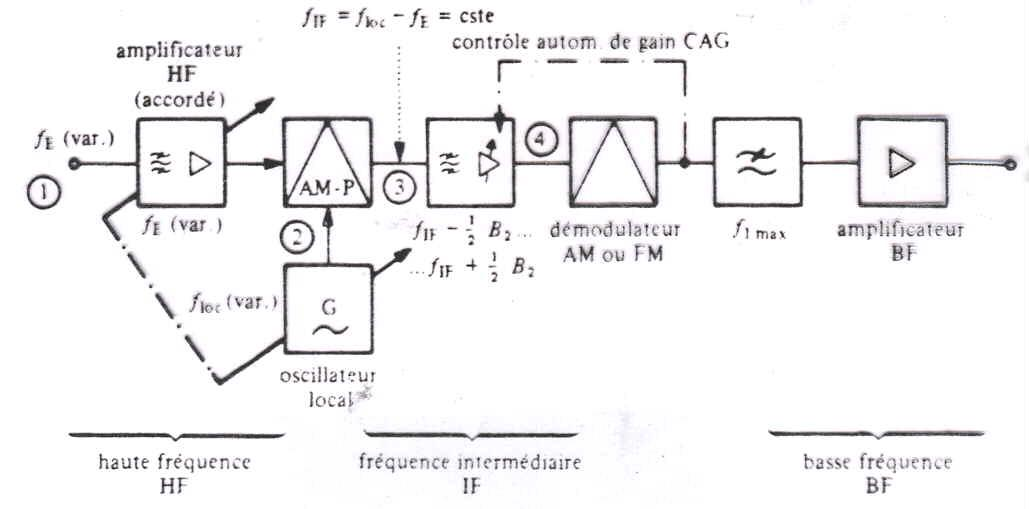
\includegraphics[width=\linewidth]{img/reception_superheterodyne.png}
    \caption{Schéma récapitulatif de la réception superhétérodyne}
\end{figure}

On reçoit un signal qui contient la fréquence sur laquelle on doit se
caler (1). Un amplificateur HF (haute fréquence) assure une première
amplification du signal (suppression du bruit utile pour les fréquences
élevées). Avec le signal provenant de l'oscillateur (2) et celui provenant
de l'antenne, on produit un signal modulé en amplitude (3). Le signal passe
ensuite dans un filtre de fréquence intermédiaire qui va supprimer
certaines composantes non-nécessaires du signal produites lors du
passage par l'étape précédente. Le signal passe par un amplificateur
responsable du gain qui contient aussi un contrôle automatique du gain
(CAG).  \newline

Le nouveau signal (4) est maintenant à un niveau nécessaire pour la
démodulation (d'amplitude ou de fréquence). Les fréquences indésirables
sont filtrées à la sortie de l'amplificateur. Le signal passe enfin par
un amplificateur basse fréquence. \newline

\subsubsection{Expliquer les principes du codage de Vernam}

Le codage de Vernam est une technique de cryptographie qui consiste à
chiffrer avec un message \og{}en clair\fg{} avec une clé présentant
certaines caractéristiques :

\begin{enumerate}
    \item La clé doit être une suite de caractères aussi longue que le
        message à chiffrer.
    \item Les caractères composant la clé doivent être choisis de façon
        totalement aléatoire.
    \item Chaque clé ne doit être utilisée qu'une seule fois (jetable)
\end{enumerate}

Si on respecte ces règles, le système offre une sécurité absolue.
L'envoyeur et le récepteur du message doivent posséder la clé et pour la
transmission de cette clé de manière totalement sûr, elle doit être
physique. Le problème de la sécurité se passe est donc physique, les
applications sont surtout militaires.
\newline

\subsubsection{En quoi consiste l'échantillonnage ?}

L'échantillonnage consiste à transmettre un signal en capturant des
valeurs à intervalles réguliers. Il produit une suite de valeurs
discrètes. Il s'utilise dans le cadre d'une numérisation d'un signal. 

\subsubsection{En quoi consiste la numérisation ?}

La numérisation est la conversion d'un signal analogique (continu)
en un signal numérique (discret). \newline

La numérisation se fait en plusieurs étapes :
\begin{enumerate}
    \item L'\textbf{échantillonnage} prélève à intervalles réguliers des valeurs
        du signal.
    \item La \textbf{quantification} transforme une valeur quelconque en une
        valeur prise dans une liste finie de valeurs valides pour le
        système.
    \item Le \textbf{codage} fait correspondre à chaque valeur valide pour le
        système un code numérique.
\end{enumerate}

Les avantages sont nombreux : ça permet un traitement informatique des
données (les ordinateurs ne peuvent traiter que des formes discrètes),
le stockage des signaux et donc leur re-création et la possibilité
d'appliquer des codes détecteurs (voire correcteurs) sur ceux-ci.
\newline

\subsubsection{Expliquez le mécanisme de démodulation d'un signal}

\begin{figure}[H]
% Schéma d'un démodulateur en tikz
\ifx\du\undefined
  \newlength{\du}
\fi
\setlength{\du}{15\unitlength}
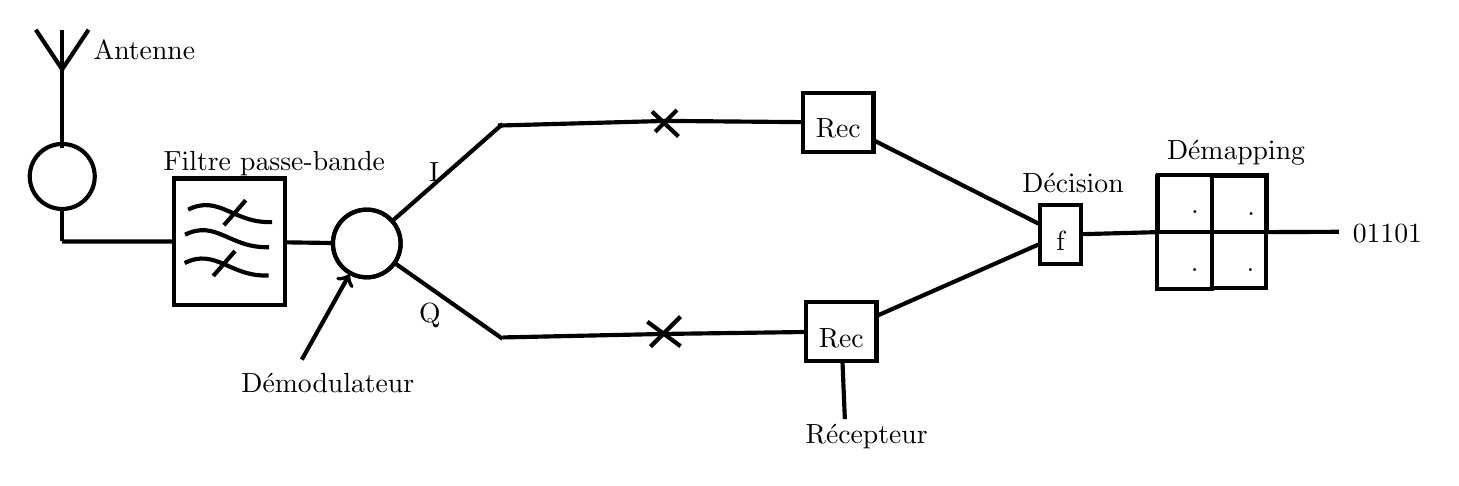
\begin{tikzpicture}[scale=0.75]
\pgftransformxscale{1.000000}
\pgftransformyscale{-1.000000}
\definecolor{dialinecolor}{rgb}{0.000000, 0.000000, 0.000000}
\pgfsetstrokecolor{dialinecolor}
\definecolor{dialinecolor}{rgb}{1.000000, 1.000000, 1.000000}
\pgfsetfillcolor{dialinecolor}
\pgfsetlinewidth{0.100000\du}
\pgfsetdash{}{0pt}
\pgfsetdash{}{0pt}
\pgfsetbuttcap
\pgfsetmiterjoin
\pgfsetlinewidth{0.100000\du}
\pgfsetbuttcap
\pgfsetmiterjoin
\pgfsetdash{}{0pt}
\definecolor{dialinecolor}{rgb}{0.000000, 0.000000, 0.000000}
\pgfsetstrokecolor{dialinecolor}
\draw (7.102782\du,6.662500\du)--(7.102782\du,4.120833\du);
\pgfsetbuttcap
\pgfsetmiterjoin
\pgfsetdash{}{0pt}
\definecolor{dialinecolor}{rgb}{0.000000, 0.000000, 0.000000}
\pgfsetstrokecolor{dialinecolor}
\draw (6.255560\du,2.850000\du)--(7.102782\du,4.120833\du);
\pgfsetbuttcap
\pgfsetmiterjoin
\pgfsetdash{}{0pt}
\definecolor{dialinecolor}{rgb}{0.000000, 0.000000, 0.000000}
\pgfsetstrokecolor{dialinecolor}
\draw (7.102782\du,2.850000\du)--(7.102782\du,4.120833\du);
\pgfsetbuttcap
\pgfsetmiterjoin
\pgfsetdash{}{0pt}
\definecolor{dialinecolor}{rgb}{0.000000, 0.000000, 0.000000}
\pgfsetstrokecolor{dialinecolor}
\draw (7.950004\du,2.850000\du)--(7.102782\du,4.120833\du);
\pgfsetlinewidth{0.100000\du}
\pgfsetdash{}{0pt}
\pgfsetdash{}{0pt}
\pgfsetbuttcap
\pgfsetmiterjoin
\pgfsetlinewidth{0.100000\du}
\pgfsetbuttcap
\pgfsetmiterjoin
\pgfsetdash{}{0pt}
\definecolor{dialinecolor}{rgb}{0.000000, 0.000000, 0.000000}
\pgfsetstrokecolor{dialinecolor}
\pgfpathellipse{\pgfpoint{7.106250\du}{7.562500\du}}{\pgfpoint{1.043750\du}{0\du}}{\pgfpoint{0\du}{1.043750\du}}
\pgfusepath{stroke}
\pgfsetbuttcap
\pgfsetmiterjoin
\pgfsetdash{}{0pt}
\definecolor{dialinecolor}{rgb}{0.000000, 0.000000, 0.000000}
\pgfsetstrokecolor{dialinecolor}
\draw (7.106250\du,6.518750\du)--(7.106250\du,5.475000\du);
\pgfsetbuttcap
\pgfsetmiterjoin
\pgfsetdash{}{0pt}
\definecolor{dialinecolor}{rgb}{0.000000, 0.000000, 0.000000}
\pgfsetstrokecolor{dialinecolor}
\draw (7.106250\du,8.606250\du)--(7.106250\du,9.650000\du);
\definecolor{dialinecolor}{rgb}{1.000000, 1.000000, 1.000000}
\pgfsetfillcolor{dialinecolor}
\fill (10.700000\du,7.627740\du)--(10.700000\du,11.677740\du)--(14.250000\du,11.677740\du)--(14.250000\du,7.627740\du)--cycle;
\pgfsetlinewidth{0.100000\du}
\pgfsetdash{}{0pt}
\pgfsetdash{}{0pt}
\pgfsetmiterjoin
\definecolor{dialinecolor}{rgb}{0.000000, 0.000000, 0.000000}
\pgfsetstrokecolor{dialinecolor}
\draw (10.700000\du,7.627740\du)--(10.700000\du,11.677740\du)--(14.250000\du,11.677740\du)--(14.250000\du,7.627740\du)--cycle;
% setfont left to latex
\definecolor{dialinecolor}{rgb}{0.000000, 0.000000, 0.000000}
\pgfsetstrokecolor{dialinecolor}
\node at (12.475000\du,9.847740\du){};
\pgfsetlinewidth{0.100000\du}
\pgfsetdash{}{0pt}
\pgfsetdash{}{0pt}
\pgfsetbuttcap
{
\definecolor{dialinecolor}{rgb}{0.000000, 0.000000, 0.000000}
\pgfsetfillcolor{dialinecolor}
% was here!!!
\definecolor{dialinecolor}{rgb}{0.000000, 0.000000, 0.000000}
\pgfsetstrokecolor{dialinecolor}
\draw (7.106250\du,9.650000\du)--(10.649809\du,9.651808\du);
}
\pgfsetlinewidth{0.100000\du}
\pgfsetdash{}{0pt}
\pgfsetdash{}{0pt}
\pgfsetmiterjoin
\pgfsetbuttcap
{
\definecolor{dialinecolor}{rgb}{0.000000, 0.000000, 0.000000}
\pgfsetfillcolor{dialinecolor}
% was here!!!
\definecolor{dialinecolor}{rgb}{0.000000, 0.000000, 0.000000}
\pgfsetstrokecolor{dialinecolor}
\pgfpathmoveto{\pgfpoint{11.150000\du}{8.627740\du}}
\pgfpathcurveto{\pgfpoint{12.150000\du}{8.127740\du}}{\pgfpoint{12.600000\du}{9.077740\du}}{\pgfpoint{13.850000\du}{9.027740\du}}
\pgfusepath{stroke}
}
\pgfsetlinewidth{0.100000\du}
\pgfsetdash{}{0pt}
\pgfsetdash{}{0pt}
\pgfsetmiterjoin
\pgfsetbuttcap
{
\definecolor{dialinecolor}{rgb}{0.000000, 0.000000, 0.000000}
\pgfsetfillcolor{dialinecolor}
% was here!!!
\definecolor{dialinecolor}{rgb}{0.000000, 0.000000, 0.000000}
\pgfsetstrokecolor{dialinecolor}
\pgfpathmoveto{\pgfpoint{11.052100\du}{9.433590\du}}
\pgfpathcurveto{\pgfpoint{12.052100\du}{8.933590\du}}{\pgfpoint{12.502100\du}{9.883590\du}}{\pgfpoint{13.752100\du}{9.833590\du}}
\pgfusepath{stroke}
}
\pgfsetlinewidth{0.100000\du}
\pgfsetdash{}{0pt}
\pgfsetdash{}{0pt}
\pgfsetmiterjoin
\pgfsetbuttcap
{
\definecolor{dialinecolor}{rgb}{0.000000, 0.000000, 0.000000}
\pgfsetfillcolor{dialinecolor}
% was here!!!
\definecolor{dialinecolor}{rgb}{0.000000, 0.000000, 0.000000}
\pgfsetstrokecolor{dialinecolor}
\pgfpathmoveto{\pgfpoint{11.037100\du}{10.343600\du}}
\pgfpathcurveto{\pgfpoint{12.037100\du}{9.843590\du}}{\pgfpoint{12.487100\du}{10.793600\du}}{\pgfpoint{13.737100\du}{10.743600\du}}
\pgfusepath{stroke}
}
\pgfsetlinewidth{0.100000\du}
\pgfsetdash{}{0pt}
\pgfsetdash{}{0pt}
\pgfsetbuttcap
{
\definecolor{dialinecolor}{rgb}{0.000000, 0.000000, 0.000000}
\pgfsetfillcolor{dialinecolor}
% was here!!!
\definecolor{dialinecolor}{rgb}{0.000000, 0.000000, 0.000000}
\pgfsetstrokecolor{dialinecolor}
\draw (13.000000\du,8.327740\du)--(12.300000\du,9.127740\du);
}
\pgfsetlinewidth{0.100000\du}
\pgfsetdash{}{0pt}
\pgfsetdash{}{0pt}
\pgfsetbuttcap
{
\definecolor{dialinecolor}{rgb}{0.000000, 0.000000, 0.000000}
\pgfsetfillcolor{dialinecolor}
% was here!!!
\definecolor{dialinecolor}{rgb}{0.000000, 0.000000, 0.000000}
\pgfsetstrokecolor{dialinecolor}
\draw (12.655600\du,9.958290\du)--(11.955600\du,10.758300\du);
}
\pgfsetlinewidth{0.100000\du}
\pgfsetdash{}{0pt}
\pgfsetdash{}{0pt}
\pgfsetbuttcap
\pgfsetmiterjoin
\pgfsetlinewidth{0.100000\du}
\pgfsetbuttcap
\pgfsetmiterjoin
\pgfsetdash{}{0pt}
\definecolor{dialinecolor}{rgb}{1.000000, 1.000000, 1.000000}
\pgfsetfillcolor{dialinecolor}
\pgfpathellipse{\pgfpoint{16.887500\du}{9.715240\du}}{\pgfpoint{1.087500\du}{0\du}}{\pgfpoint{0\du}{1.087500\du}}
\pgfusepath{fill}
\definecolor{dialinecolor}{rgb}{0.000000, 0.000000, 0.000000}
\pgfsetstrokecolor{dialinecolor}
\pgfpathellipse{\pgfpoint{16.887500\du}{9.715240\du}}{\pgfpoint{1.087500\du}{0\du}}{\pgfpoint{0\du}{1.087500\du}}
\pgfusepath{stroke}
\pgfsetbuttcap
\pgfsetmiterjoin
\pgfsetdash{}{0pt}
\definecolor{dialinecolor}{rgb}{0.000000, 0.000000, 0.000000}
\pgfsetstrokecolor{dialinecolor}
\pgfpathellipse{\pgfpoint{16.887500\du}{9.715240\du}}{\pgfpoint{1.087500\du}{0\du}}{\pgfpoint{0\du}{1.087500\du}}
\pgfusepath{stroke}
\pgfsetlinewidth{0.100000\du}
\pgfsetdash{}{0pt}
\pgfsetdash{}{0pt}
\pgfsetbuttcap
{
\definecolor{dialinecolor}{rgb}{0.000000, 0.000000, 0.000000}
\pgfsetfillcolor{dialinecolor}
% was here!!!
\definecolor{dialinecolor}{rgb}{0.000000, 0.000000, 0.000000}
\pgfsetstrokecolor{dialinecolor}
\draw (14.300435\du,9.678596\du)--(15.767139\du,9.699371\du);
}
\pgfsetlinewidth{0.100000\du}
\pgfsetdash{}{0pt}
\pgfsetdash{}{0pt}
\pgfsetbuttcap
{
\definecolor{dialinecolor}{rgb}{0.000000, 0.000000, 0.000000}
\pgfsetfillcolor{dialinecolor}
% was here!!!
\definecolor{dialinecolor}{rgb}{0.000000, 0.000000, 0.000000}
\pgfsetstrokecolor{dialinecolor}
\draw (17.740616\du,8.964791\du)--(21.250000\du,5.877740\du);
}
\pgfsetlinewidth{0.100000\du}
\pgfsetdash{}{0pt}
\pgfsetdash{}{0pt}
\pgfsetbuttcap
{
\definecolor{dialinecolor}{rgb}{0.000000, 0.000000, 0.000000}
\pgfsetfillcolor{dialinecolor}
% was here!!!
\definecolor{dialinecolor}{rgb}{0.000000, 0.000000, 0.000000}
\pgfsetstrokecolor{dialinecolor}
\draw (17.818632\du,10.368891\du)--(21.250000\du,12.777700\du);
}
\pgfsetlinewidth{0.100000\du}
\pgfsetdash{}{0pt}
\pgfsetdash{}{0pt}
\pgfsetbuttcap
{
\definecolor{dialinecolor}{rgb}{0.000000, 0.000000, 0.000000}
\pgfsetfillcolor{dialinecolor}
% was here!!!
\definecolor{dialinecolor}{rgb}{0.000000, 0.000000, 0.000000}
\pgfsetstrokecolor{dialinecolor}
\draw (26.850000\du,5.427740\du)--(26.150000\du,6.127740\du);
}
\pgfsetlinewidth{0.100000\du}
\pgfsetdash{}{0pt}
\pgfsetdash{}{0pt}
\pgfsetbuttcap
{
\definecolor{dialinecolor}{rgb}{0.000000, 0.000000, 0.000000}
\pgfsetfillcolor{dialinecolor}
% was here!!!
\definecolor{dialinecolor}{rgb}{0.000000, 0.000000, 0.000000}
\pgfsetstrokecolor{dialinecolor}
\draw (26.050000\du,5.477740\du)--(26.900000\du,6.277740\du);
}
\pgfsetlinewidth{0.100000\du}
\pgfsetdash{}{0pt}
\pgfsetdash{}{0pt}
\pgfsetbuttcap
{
\definecolor{dialinecolor}{rgb}{0.000000, 0.000000, 0.000000}
\pgfsetfillcolor{dialinecolor}
% was here!!!
\definecolor{dialinecolor}{rgb}{0.000000, 0.000000, 0.000000}
\pgfsetstrokecolor{dialinecolor}
\draw (26.965700\du,12.063400\du)--(26.000000\du,13.027700\du);
}
\pgfsetlinewidth{0.100000\du}
\pgfsetdash{}{0pt}
\pgfsetdash{}{0pt}
\pgfsetbuttcap
{
\definecolor{dialinecolor}{rgb}{0.000000, 0.000000, 0.000000}
\pgfsetfillcolor{dialinecolor}
% was here!!!
\definecolor{dialinecolor}{rgb}{0.000000, 0.000000, 0.000000}
\pgfsetstrokecolor{dialinecolor}
\draw (25.900000\du,12.227700\du)--(26.965700\du,13.013400\du);
}
\pgfsetlinewidth{0.100000\du}
\pgfsetdash{}{0pt}
\pgfsetdash{}{0pt}
\pgfsetbuttcap
{
\definecolor{dialinecolor}{rgb}{0.000000, 0.000000, 0.000000}
\pgfsetfillcolor{dialinecolor}
% was here!!!
\definecolor{dialinecolor}{rgb}{0.000000, 0.000000, 0.000000}
\pgfsetstrokecolor{dialinecolor}
\draw (21.100000\du,5.927740\du)--(26.500000\du,5.777740\du);
}
\pgfsetlinewidth{0.100000\du}
\pgfsetdash{}{0pt}
\pgfsetdash{}{0pt}
\pgfsetbuttcap
{
\definecolor{dialinecolor}{rgb}{0.000000, 0.000000, 0.000000}
\pgfsetfillcolor{dialinecolor}
% was here!!!
\definecolor{dialinecolor}{rgb}{0.000000, 0.000000, 0.000000}
\pgfsetstrokecolor{dialinecolor}
\draw (21.256500\du,12.732700\du)--(26.432800\du,12.620600\du);
}
\definecolor{dialinecolor}{rgb}{1.000000, 1.000000, 1.000000}
\pgfsetfillcolor{dialinecolor}
\fill (30.900000\du,4.877740\du)--(30.900000\du,6.777740\du)--(33.165000\du,6.777740\du)--(33.165000\du,4.877740\du)--cycle;
\pgfsetlinewidth{0.100000\du}
\pgfsetdash{}{0pt}
\pgfsetdash{}{0pt}
\pgfsetmiterjoin
\definecolor{dialinecolor}{rgb}{0.000000, 0.000000, 0.000000}
\pgfsetstrokecolor{dialinecolor}
\draw (30.900000\du,4.877740\du)--(30.900000\du,6.777740\du)--(33.165000\du,6.777740\du)--(33.165000\du,4.877740\du)--cycle;
% setfont left to latex
\definecolor{dialinecolor}{rgb}{0.000000, 0.000000, 0.000000}
\pgfsetstrokecolor{dialinecolor}
\node at (32.032500\du,6.022740\du){Rec};
\definecolor{dialinecolor}{rgb}{1.000000, 1.000000, 1.000000}
\pgfsetfillcolor{dialinecolor}
\fill (30.995000\du,11.592700\du)--(30.995000\du,13.492700\du)--(33.260000\du,13.492700\du)--(33.260000\du,11.592700\du)--cycle;
\pgfsetlinewidth{0.100000\du}
\pgfsetdash{}{0pt}
\pgfsetdash{}{0pt}
\pgfsetmiterjoin
\definecolor{dialinecolor}{rgb}{0.000000, 0.000000, 0.000000}
\pgfsetstrokecolor{dialinecolor}
\draw (30.995000\du,11.592700\du)--(30.995000\du,13.492700\du)--(33.260000\du,13.492700\du)--(33.260000\du,11.592700\du)--cycle;
% setfont left to latex
\definecolor{dialinecolor}{rgb}{0.000000, 0.000000, 0.000000}
\pgfsetstrokecolor{dialinecolor}
\node at (32.127500\du,12.737700\du){Rec};
\pgfsetlinewidth{0.100000\du}
\pgfsetdash{}{0pt}
\pgfsetdash{}{0pt}
\pgfsetbuttcap
{
\definecolor{dialinecolor}{rgb}{0.000000, 0.000000, 0.000000}
\pgfsetfillcolor{dialinecolor}
% was here!!!
\definecolor{dialinecolor}{rgb}{0.000000, 0.000000, 0.000000}
\pgfsetstrokecolor{dialinecolor}
\draw (26.500000\du,5.777740\du)--(30.851981\du,5.817071\du);
}
\pgfsetlinewidth{0.100000\du}
\pgfsetdash{}{0pt}
\pgfsetdash{}{0pt}
\pgfsetbuttcap
{
\definecolor{dialinecolor}{rgb}{0.000000, 0.000000, 0.000000}
\pgfsetfillcolor{dialinecolor}
% was here!!!
\definecolor{dialinecolor}{rgb}{0.000000, 0.000000, 0.000000}
\pgfsetstrokecolor{dialinecolor}
\draw (30.945043\du,12.558875\du)--(26.432800\du,12.620600\du);
}
\definecolor{dialinecolor}{rgb}{1.000000, 1.000000, 1.000000}
\pgfsetfillcolor{dialinecolor}
\fill (38.509900\du,8.485040\du)--(38.509900\du,10.385040\du)--(39.834900\du,10.385040\du)--(39.834900\du,8.485040\du)--cycle;
\pgfsetlinewidth{0.100000\du}
\pgfsetdash{}{0pt}
\pgfsetdash{}{0pt}
\pgfsetmiterjoin
\definecolor{dialinecolor}{rgb}{0.000000, 0.000000, 0.000000}
\pgfsetstrokecolor{dialinecolor}
\draw (38.509900\du,8.485040\du)--(38.509900\du,10.385040\du)--(39.834900\du,10.385040\du)--(39.834900\du,8.485040\du)--cycle;
% setfont left to latex
\definecolor{dialinecolor}{rgb}{0.000000, 0.000000, 0.000000}
\pgfsetstrokecolor{dialinecolor}
\node at (39.172400\du,9.630040\du){f};
\pgfsetlinewidth{0.100000\du}
\pgfsetdash{}{0pt}
\pgfsetdash{}{0pt}
\pgfsetbuttcap
\pgfsetmiterjoin
\pgfsetlinewidth{0.100000\du}
\pgfsetbuttcap
\pgfsetmiterjoin
\pgfsetdash{}{0pt}
\definecolor{dialinecolor}{rgb}{1.000000, 1.000000, 1.000000}
\pgfsetfillcolor{dialinecolor}
\fill (42.282000\du,7.547050\du)--(42.282000\du,11.153605\du)--(45.772215\du,11.153605\du)--(45.772215\du,7.547050\du)--cycle;
\definecolor{dialinecolor}{rgb}{0.000000, 0.000000, 0.000000}
\pgfsetstrokecolor{dialinecolor}
\draw (42.282000\du,7.547050\du)--(42.282000\du,11.153605\du)--(45.772215\du,11.153605\du)--(45.772215\du,7.547050\du)--cycle;
\pgfsetbuttcap
\pgfsetmiterjoin
\pgfsetdash{}{0pt}
\definecolor{dialinecolor}{rgb}{0.000000, 0.000000, 0.000000}
\pgfsetstrokecolor{dialinecolor}
\draw (42.282000\du,7.547050\du)--(42.282000\du,11.153605\du)--(45.772215\du,11.153605\du)--(45.772215\du,7.547050\du)--cycle;
\pgfsetlinewidth{0.100000\du}
\pgfsetdash{}{0pt}
\pgfsetdash{}{0pt}
\pgfsetbuttcap
\pgfsetmiterjoin
\pgfsetlinewidth{0.100000\du}
\pgfsetbuttcap
\pgfsetmiterjoin
\pgfsetdash{}{0pt}
\definecolor{dialinecolor}{rgb}{1.000000, 1.000000, 1.000000}
\pgfsetfillcolor{dialinecolor}
\fill (42.293700\du,7.527770\du)--(42.293700\du,9.347042\du)--(44.054286\du,9.347042\du)--(44.054286\du,7.527770\du)--cycle;
\definecolor{dialinecolor}{rgb}{0.000000, 0.000000, 0.000000}
\pgfsetstrokecolor{dialinecolor}
\draw (42.293700\du,7.527770\du)--(42.293700\du,9.347042\du)--(44.054286\du,9.347042\du)--(44.054286\du,7.527770\du)--cycle;
\pgfsetbuttcap
\pgfsetmiterjoin
\pgfsetdash{}{0pt}
\definecolor{dialinecolor}{rgb}{0.000000, 0.000000, 0.000000}
\pgfsetstrokecolor{dialinecolor}
\draw (42.293700\du,7.527770\du)--(42.293700\du,9.347042\du)--(44.054286\du,9.347042\du)--(44.054286\du,7.527770\du)--cycle;
\pgfsetlinewidth{0.100000\du}
\pgfsetdash{}{0pt}
\pgfsetdash{}{0pt}
\pgfsetbuttcap
\pgfsetmiterjoin
\pgfsetlinewidth{0.100000\du}
\pgfsetbuttcap
\pgfsetmiterjoin
\pgfsetdash{}{0pt}
\definecolor{dialinecolor}{rgb}{1.000000, 1.000000, 1.000000}
\pgfsetfillcolor{dialinecolor}
\fill (42.280200\du,9.344450\du)--(42.280200\du,11.170190\du)--(44.047045\du,11.170190\du)--(44.047045\du,9.344450\du)--cycle;
\definecolor{dialinecolor}{rgb}{0.000000, 0.000000, 0.000000}
\pgfsetstrokecolor{dialinecolor}
\draw (42.280200\du,9.344450\du)--(42.280200\du,11.170190\du)--(44.047045\du,11.170190\du)--(44.047045\du,9.344450\du)--cycle;
\pgfsetbuttcap
\pgfsetmiterjoin
\pgfsetdash{}{0pt}
\definecolor{dialinecolor}{rgb}{0.000000, 0.000000, 0.000000}
\pgfsetstrokecolor{dialinecolor}
\draw (42.280200\du,9.344450\du)--(42.280200\du,11.170190\du)--(44.047045\du,11.170190\du)--(44.047045\du,9.344450\du)--cycle;
\pgfsetlinewidth{0.100000\du}
\pgfsetdash{}{0pt}
\pgfsetdash{}{0pt}
\pgfsetbuttcap
\pgfsetmiterjoin
\pgfsetlinewidth{0.100000\du}
\pgfsetbuttcap
\pgfsetmiterjoin
\pgfsetdash{}{0pt}
\definecolor{dialinecolor}{rgb}{1.000000, 1.000000, 1.000000}
\pgfsetfillcolor{dialinecolor}
\fill (44.040600\du,7.531510\du)--(44.040600\du,9.337163\du)--(45.788006\du,9.337163\du)--(45.788006\du,7.531510\du)--cycle;
\definecolor{dialinecolor}{rgb}{0.000000, 0.000000, 0.000000}
\pgfsetstrokecolor{dialinecolor}
\draw (44.040600\du,7.531510\du)--(44.040600\du,9.337163\du)--(45.788006\du,9.337163\du)--(45.788006\du,7.531510\du)--cycle;
\pgfsetbuttcap
\pgfsetmiterjoin
\pgfsetdash{}{0pt}
\definecolor{dialinecolor}{rgb}{0.000000, 0.000000, 0.000000}
\pgfsetstrokecolor{dialinecolor}
\draw (44.040600\du,7.531510\du)--(44.040600\du,9.337163\du)--(45.788006\du,9.337163\du)--(45.788006\du,7.531510\du)--cycle;
% setfont left to latex
\definecolor{dialinecolor}{rgb}{0.000000, 0.000000, 0.000000}
\pgfsetstrokecolor{dialinecolor}
\node[anchor=west] at (43.000500\du,8.707300\du){.};
% setfont left to latex
\definecolor{dialinecolor}{rgb}{0.000000, 0.000000, 0.000000}
\pgfsetstrokecolor{dialinecolor}
\node[anchor=west] at (44.811800\du,8.764720\du){.};
% setfont left to latex
\definecolor{dialinecolor}{rgb}{0.000000, 0.000000, 0.000000}
\pgfsetstrokecolor{dialinecolor}
\node[anchor=west] at (42.997800\du,10.563300\du){.};
% setfont left to latex
\definecolor{dialinecolor}{rgb}{0.000000, 0.000000, 0.000000}
\pgfsetstrokecolor{dialinecolor}
\node[anchor=west] at (44.788600\du,10.569100\du){.};
\pgfsetlinewidth{0.100000\du}
\pgfsetdash{}{0pt}
\pgfsetdash{}{0pt}
\pgfsetbuttcap
{
\definecolor{dialinecolor}{rgb}{0.000000, 0.000000, 0.000000}
\pgfsetfillcolor{dialinecolor}
% was here!!!
\definecolor{dialinecolor}{rgb}{0.000000, 0.000000, 0.000000}
\pgfsetstrokecolor{dialinecolor}
\draw (33.297063\du,12.026780\du)--(38.459912\du,9.749334\du);
}
\pgfsetlinewidth{0.100000\du}
\pgfsetdash{}{0pt}
\pgfsetdash{}{0pt}
\pgfsetbuttcap
{
\definecolor{dialinecolor}{rgb}{0.000000, 0.000000, 0.000000}
\pgfsetfillcolor{dialinecolor}
% was here!!!
\definecolor{dialinecolor}{rgb}{0.000000, 0.000000, 0.000000}
\pgfsetstrokecolor{dialinecolor}
\draw (33.214784\du,6.425067\du)--(38.460327\du,9.075279\du);
}
\pgfsetlinewidth{0.100000\du}
\pgfsetdash{}{0pt}
\pgfsetdash{}{0pt}
\pgfsetbuttcap
{
\definecolor{dialinecolor}{rgb}{0.000000, 0.000000, 0.000000}
\pgfsetfillcolor{dialinecolor}
% was here!!!
\definecolor{dialinecolor}{rgb}{0.000000, 0.000000, 0.000000}
\pgfsetstrokecolor{dialinecolor}
\draw (39.884890\du,9.415631\du)--(42.282000\du,9.350330\du);
}
\pgfsetlinewidth{0.100000\du}
\pgfsetdash{}{0pt}
\pgfsetdash{}{0pt}
\pgfsetbuttcap
{
\definecolor{dialinecolor}{rgb}{0.000000, 0.000000, 0.000000}
\pgfsetfillcolor{dialinecolor}
% was here!!!
\definecolor{dialinecolor}{rgb}{0.000000, 0.000000, 0.000000}
\pgfsetstrokecolor{dialinecolor}
\draw (45.772300\du,9.350330\du)--(48.109700\du,9.339400\du);
}
% setfont left to latex
\definecolor{dialinecolor}{rgb}{0.000000, 0.000000, 0.000000}
\pgfsetstrokecolor{dialinecolor}
\node[anchor=west] at (18.529300\du,7.414790\du){I};
% setfont left to latex
\definecolor{dialinecolor}{rgb}{0.000000, 0.000000, 0.000000}
\pgfsetstrokecolor{dialinecolor}
\node[anchor=west] at (18.205100\du,12.051000\du){Q};
\pgfsetlinewidth{0.100000\du}
\pgfsetdash{}{0pt}
\pgfsetdash{}{0pt}
\pgfsetbuttcap
{
\definecolor{dialinecolor}{rgb}{0.000000, 0.000000, 0.000000}
\pgfsetfillcolor{dialinecolor}
% was here!!!
\pgfsetarrowsend{to}
\definecolor{dialinecolor}{rgb}{0.000000, 0.000000, 0.000000}
\pgfsetstrokecolor{dialinecolor}
\draw (14.800900\du,13.445100\du)--(16.331973\du,10.708261\du);
}
% setfont left to latex
\definecolor{dialinecolor}{rgb}{0.000000, 0.000000, 0.000000}
\pgfsetstrokecolor{dialinecolor}
\node[anchor=west] at (12.499000\du,14.190800\du){Démodulateur};
\pgfsetlinewidth{0.100000\du}
\pgfsetdash{}{0pt}
\pgfsetdash{}{0pt}
\pgfsetbuttcap
{
\definecolor{dialinecolor}{rgb}{0.000000, 0.000000, 0.000000}
\pgfsetfillcolor{dialinecolor}
% was here!!!
\definecolor{dialinecolor}{rgb}{0.000000, 0.000000, 0.000000}
\pgfsetstrokecolor{dialinecolor}
\draw (32.168437\du,13.537917\du)--(32.243300\du,15.357900\du);
}
% setfont left to latex
\definecolor{dialinecolor}{rgb}{0.000000, 0.000000, 0.000000}
\pgfsetstrokecolor{dialinecolor}
\node[anchor=west] at (30.622300\du,15.909100\du){Récepteur};
% setfont left to latex
\definecolor{dialinecolor}{rgb}{0.000000, 0.000000, 0.000000}
\pgfsetstrokecolor{dialinecolor}
\node[anchor=west] at (37.583400\du,7.760470\du){Décision};
% setfont left to latex
\definecolor{dialinecolor}{rgb}{0.000000, 0.000000, 0.000000}
\pgfsetstrokecolor{dialinecolor}
\node[anchor=west] at (42.229000\du,6.798790\du){Démapping};
% setfont left to latex
\definecolor{dialinecolor}{rgb}{0.000000, 0.000000, 0.000000}
\pgfsetstrokecolor{dialinecolor}
\node[anchor=west] at (48.194400\du,9.392460\du){01101};
% setfont left to latex
\definecolor{dialinecolor}{rgb}{0.000000, 0.000000, 0.000000}
\pgfsetstrokecolor{dialinecolor}
\node[anchor=west] at (7.750000\du,3.500000\du){Antenne};
% setfont left to latex
\definecolor{dialinecolor}{rgb}{0.000000, 0.000000, 0.000000}
\pgfsetstrokecolor{dialinecolor}
\node[anchor=west] at (10.000000\du,7.150000\du){Filtre passe-bande};
\end{tikzpicture}

\caption{Schéma d'un démodulateur}
\end{figure}

L'antenne ou un autre récepteur permet de réceptionner un signal modulé qui va
passer au travers d'un filtre (passe-bande, passe-haut, passe-bas) pour
ne garder que la partie du signal qui nous intéresse (resp. une bande de
fréquence, les hautes fréquences, les basses fréquences). Le modulateur
et le démodulateur doivent partager la même porteuse ou un signal
permettant de la retrouver. On filtre le signal de manière à retrouver
son enveloppe. Le passage dans le démodulateur sépare le
signal entre la partie réelle et la partie imaginaire. \newline

Le récepteur traite la partie réelle et complexe et à travers un
processus de décision prédéfini on va replacer les valeurs sur la
constellation (c'est le démapping). \newline

\subsubsection{Décrivez la structure du réseau GSM}

\begin{figure}[H]
    \centering
    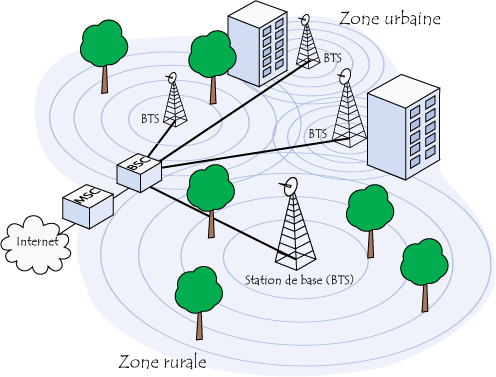
\includegraphics[width=\linewidth]{img/structure_reseau_gsm.png}
    \caption{Structure du réseau GSM}
\end{figure}

Le réseau est composé de nombreux BTS (Base Transceiver System : antennes et équipement qui
couvrent une cellule) qui sont connectés entre eux à travers des BSC
(Base Station Controller) eux-mêmes reliés à des MSC (Mobile Switching
Center) qui transmettent à travers Internet les appels aux réseaux fixes
et GSM concurrents. \newline

\subsection{Exercices}

Formules utiles :

\begin{itemize}
\item[$P_{T_i}$] Puissance émetteur isotrope équivalente
\item[$P_{R_i}$] Puissance récepteur isotrope équivalente
\item[$P_T$] Puissance émetteur
\item[$G_T$] Gain émetteur
\item[$P_R$] Puissance récepteur
\item[$G_R$] Gain Récepteur
\item[$L_c$] Pertes dans le cable
\item[$L_{FS}$] Perte dans l'air
\item[$D$] portée (durant le cours c'est $r$, le rayon isotrope
\item[$A$] Air effective de l'antenne
\end{itemize}

$$P_{T_i} = \frac{P_TG_T}{L_c}$$
$$L_{FS} = \left(\frac{4\pi D}{\lambda}\right)^2$$
Dans la formule suivante, si il s'agit d'une parabole on doit multiplier les pertes au dénominateur par $\theta$ (les pertes causé par la pluie, la moisisure, les gaz, ...).
$$P_R = P_{T_i}G_R \left(\frac{\lambda}{4\pi D}\right)^2=\frac{P_{T_i}G_R}{L_{FS}}$$
$$P_R = \frac{A}{4\pi D^2}P_TG_T$$
$$P_R = P_{R_i}G_R$$

\subsubsection*{Si ma ligne atténue le signal d'un facteur de 10000 en puissance sur 1km,
quelle est le facteur d'atténuation en dB/m? }

Un facteur de $10000$ par kilomètre correspond à un facteur de 10 en
mètres.

\[ 10log(10) = 10[dB\div m] \]

\subsubsection*{Si j'utilise un récepteur super hétérodyne avec une fréquence intermédiaire
  de 20kHz, quelle doit être la fréquence de l'oscillateur local pour recevoir
une station à 100kHz? Quelle est la fréquence image?}



\subsubsection*{Illustrez la compression par Lempel-Ziv de la séquence suivante :
  ``01001100000110110110'', à partir du 6\up{ème} bit.}
